\chapter{一些细节的问题}

\section{模板文件结构及功能介绍}

模板文件的结构与功能, 如下表所示:
\begin{table}[ht]\centering
    \begin{tabular}{lll}
        \toprule
        文件夹/文件名                             & 类型     & 功能说明                \\
        \midrule
        gdufe\_master\_thesis\_template.tex & 主文档    & 撰写正文、组织结构           \\
        gdufe\_master\_thesis.cls           & 类文件    & 定义排版格式和命令           \\
        reference.bib                       & bib文件  & 参考文献数据库             \\
        README.md                           & 文本     & 项目说明与使用方法           \\
        includefile/                        & 文件夹    & 存放各章节、摘要、致谢等        \\
        \quad abstract.tex                  & tex文件  & 中英文摘要               \\
        \quad acknowledgment.tex            & tex文件  & 致谢                  \\
        \quad 论文封面、扉页及声明格式.doc              & Word文档 & 编写封面、扉页及声明页         \\
        \quad 论文封面、扉页及声明格式.pdf              & PDF    & 用于编译Tex文件的封面、扉页及声明页 \\
        figures/                            & 文件夹    & 存放图片文件              \\
        \quad gdufelogo.jpg                 & 图片     & 校徽图片                \\
        fonts/                              & 文件夹    & 存放字体文件              \\
        \quad 仿宋\_gb2312.ttf                & 字体     & 仿宋字体                \\
        \bottomrule
    \end{tabular}
    \caption{模板文件结构及功能说明}
\end{table}

无需也不要改变、移动上述文档的位置.

如果不习惯用~\verb|\include{ }|~的方式加入``子文档'', 当然可以把它们合并在主文档, 成为一个文档.
({\kaishu 但是这样并不会给我们带来方便.})

利用~WinEdt~的~Project tree(如图~\ref{fig:1} ), 可以方便地管理这些文件.
\begin{figure}[h]
    \centering
    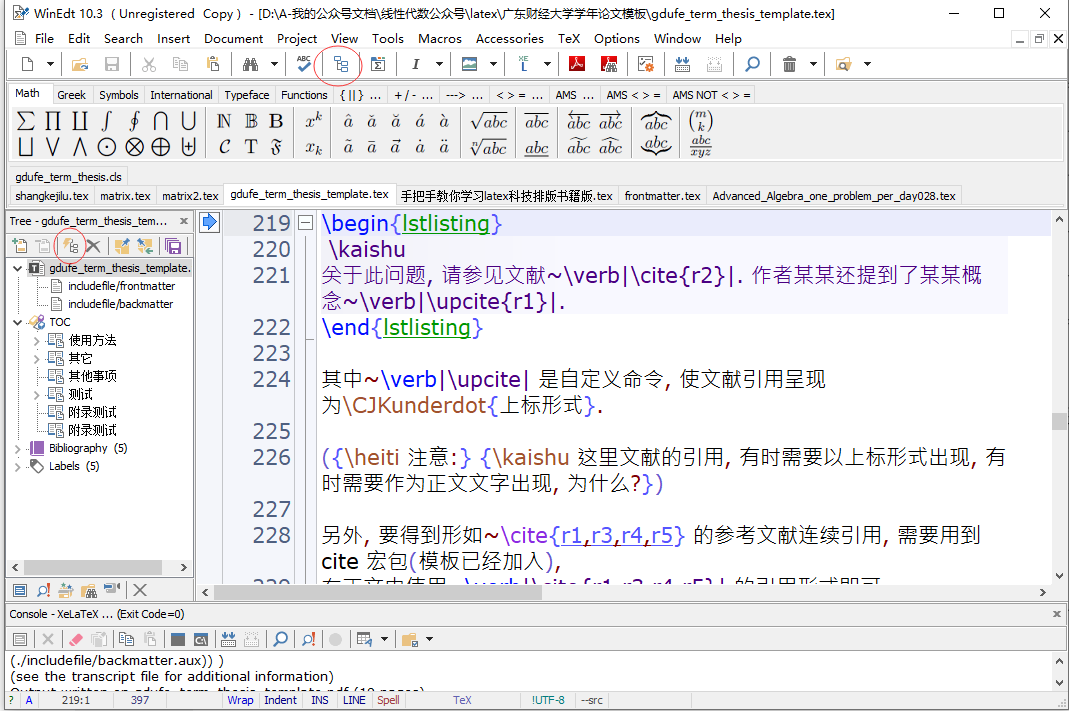
\includegraphics[width=\textwidth]{winedt_file_tree.png}
    \caption{方便在文档内定位的大纲树图}
    \label{fig:1}
\end{figure}

\begin{itemize}
    \item 点击~WinEdt~窗口的~Project Tree~按键;
    \item 再点击~WinEdt~窗口的~Set Main File~按键;
\end{itemize}
接下来的管理, 已经清楚地展示在跳出的窗口中了. 再去处理其他的文件时, 还要点击~WinEdt~窗口的~Remove Main File~按键.

\section{字体调节}

\begin{tabular}{ll}
    \verb|\songti|   & {\songti 宋体}   \\
    \verb|\heiti|    & {\heiti 黑体}    \\
    \verb|\fangsong| & {\fangsong 仿宋} \\
    \verb|\kaishu|   & {\kaishu 楷书}
\end{tabular}


\section{字号调节}
字号命令: \verb|\zihao| \index{zihao}

\begin{tabular}{ll}
    \verb|\zihao{0}|  & \zihao{0}  初号字 English \\
    \verb|\zihao{-0}| & \zihao{-0} 小初号 English \\
    \verb|\zihao{1} | & \zihao{1}  一号字 English \\
    \verb|\zihao{-1}| & \zihao{-1} 小一号 English \\
    \verb|\zihao{2} | & \zihao{2}  二号字 English \\
    \verb|\zihao{-2}| & \zihao{-2} 小二号 English \\
    \verb|\zihao{3} | & \zihao{3}  三号字 English \\
    \verb|\zihao{-3}| & \zihao{-3} 小三号 English \\
    \verb|\zihao{4} | & \zihao{4}  四号字 English \\
    \verb|\zihao{-4}| & \zihao{-4} 小四号 English \\
    \verb|\zihao{5} | & \zihao{5}  五号字 English \\
    \verb|\zihao{-5}| & \zihao{-5} 小五号 English \\
    \verb|\zihao{6} | & \zihao{6}  六号字 English \\
    \verb|\zihao{-6}| & \zihao{-6} 小六号 English \\
    \verb|\zihao{7} | & \zihao{7}  七号字 English \\
    \verb|\zihao{8} | & \zihao{8}  八号字 English \\
\end{tabular}

\section{已加入的常用宏包}
了解类文件cls中已经加载的宏包,在主文档中无须重复加载。
\begin{description}
    \item[amsmath,amssymb]
    \item[cite]  参考文献引用, 得到形如 [3-7] 合并引用文献的样式.
    \item[color,xcolor]  支持彩色.
    \item[enumerate]  方便自由选择 enumerate 环境的编号方式. 比如

          \verb|\begin{enumerate}[(a)]| 得到形如 (a), (b), (c) 的编号.


          \verb|\begin{enumerate}[i)]| 得到形如 i), ii), iii) 的编号.
    \item[tikz] 方便使用tikz作图功能.
    \item[listings] 方便在文档中插入各种程序代码。

\end{description}

另外要说明的是,  itemize, enumerate, description 这三种 list 环境, 已经调节了其间距和缩进,
以符合中文书写的习惯.

\section{标点符号的问题}

建议使用半角的标点符号, 后边再键入一个空格. 特别是在英文书写中要注意此问题!

双引号是由两个左单引号、两个右单引号构成的: \verb|``  ''|. 左单引号在键盘上数字~1 的左边.

但是, 无论您偏向于全角或半角, 强烈建议您使用实心的句号, 只要您书写的是自然科学的文章.
原因可能是因为, 比如使用全角句号的句子结尾处的``$x$。''容易误为数学式~$x_0$(\verb|$x_0$|)吧.



\section{交叉引用的问题}

首先要说明的是,为了得到正确的引用结果,要将tex主文档编译多次。交叉引用是\LaTeX 的强项,它的原理是为被引用对象(图、表、公式、定理等)设置一个标签,例如:~\verb|\label{<标签名>}|, 然后在需要引用的地方用 ~\verb|\ref{<标签名>}|, 就能得到被引用对象的数字编号.
\subsection{参考文献的引用}
 Zotero 软件和期刊网站大多支持导出bib文件, 因此使用 biblatex 和 bib 文件管理参考文献更加方便. 其一可以自动将参考文献表格式按gb7714-2015标准排版. 其二不需要考虑增删移动参考文献位置后重新调整参考文献表. 对此方案不熟悉可以调整回用 {thebibliography} 环境或者自己喜欢的方案.

 {\bfseries 注意:} biblatex 和 cite 包不能同时使用以下两个方案只能选择一个.

\subsubsection{使用 biblatex 管理参考文献}
使用此方案务必取消注释文件开头的\\
\verb|\usepackage[style=gb7714-2015, backend=biber]{biblatex}|\\
\verb|\addbibresource{reference.bib}|\\
以及末尾的\\
\verb|\printbibliography|\\
以及将文件开头的\\
\verb|\usepackage{cite}|\\
\verb|\newcommand{\upcite}|\\
添加注释. 此时可以使用\verb|\cite{}, \parencite{}|引用参考文献

\begin{lstlisting}
详见文献\cite{r1}\parencite{r2}
另见文献\cite[49]{r3}\parencite[106]{r4}
\end{lstlisting}

详见文献\cite{r1}\parencite{r2}
另见文献\cite[49]{r3}\parencite[106]{r4}


使用 \verb|\cite \parencite| 的参考文献是顺序编码制, 其余的引用方式请参考 biblatex, biblatex-gb7714-2015 的文档.


\subsubsection{手写 thebibliography 参考文献}
不想使用 biblatex 管理参考文献, 要得到形如~{\cite{r1,r3,r4,r5}} 的参考文献连续引用, 需要用到 cite 宏包. 但cite宏包和biblatex宏包有冲突, 因此使用此方案务必注释文件开头的\\
\verb|\usepackage[style=gb7714-2015, backend=biber]{biblatex}|\\
\verb|\addbibresource{reference.bib}|\\
以及末尾的\\
\verb|\printbibliography|\\
以及将文件开头的\\
\verb|\usepackage{cite}|\\
\verb|\newcommand{\upcite}|\\
取消注释.

此时的~\verb|\cite{r1,r3,r4,r5}|不是上标引用, 而是正文引用. 想要上标引用可以使用新定义的upcite命令, 如下:
\begin{lstlisting}
    \upcite{r1,r3,r4,r5}
\end{lstlisting}
由于冲突的问题, 请自行查看.


\subsection{定理环境和公式的引用}

本模板定义了7中新定理环境样式, 包括:定理(theorem)、定义(definition)、引理(lemma)、推论(corollary)、例(example)、注(remark). 使用时用如下的格式:
\begin{lstlisting}
\begin{<环境名>}

\end{<环境名>}
\end{lstlisting}

上面的环境名一律是这些英文单词的前四个字母,参见下面的各例:

\begin{theo}[谁发现的]\label{th-abcd}
    最大的正整数是~$1$.
\end{theo}

其源文件如下:

\begin{lstlisting}
 \begin{theo}[谁发现的]\label{th-abcd}
最大的正整数是~$1$.
\end{theo}
\end{lstlisting}

其它环境就不一一举例了。

本模板还提供了证明和解的环境. 证明的环境名为:proof, 解的环境名为solu.

\begin{proof}
    要找到这个最大的正整数, 我们设最大的正整数为~$x$, 则~$x \geqslant 1$, 两边同时乘以~$x$, 得到
    \begin{equation}\label{eq-abc}
        x^2 \geqslant x.
    \end{equation}
    而~$x$ 是最大的正整数, 由~\ref{eq-abc} 式得到
    \[
        x^2 = x.
    \]
    所以
    \begin{equation*}
        x = 1.
    \end{equation*}
\end{proof}

定理~\ref{th-abcd} 是一个重大的发现.

%%%%----- 定义等环境的举例 --------
\begin{defi}[整数]
    正整数(例如 1, 2, 3)、负整数(例如 ${-1}$, $-2$, $-3$)与零(0)合起来统称为{\heiti 整数}.
\end{defi}

\begin{rema}
    整数集合在数学上通常表示为 $\mathbf{Z}$ 或 $\mathbb{Z}$, 该记号源于德语单词 Zahlen(意为``数'')的首字母.
\end{rema}

\begin{prop}
    任意两个整数相加、相减、相乘的结果, 仍然是整数.
\end{prop}

\begin{exam}
    $1+2=3$.
\end{exam}

\begin{coro}
    在整数集合内, 相加、相减、相乘运算是封闭的.
\end{coro}

\section{图形}

支持对~eps, pdf, jpg 等等常见图形格式.

再次\colorbox{red!45}{澄清一个误会}: \LaTeX{} 支持的图形格式绝非 eps 这一种. 无需特意把图片转化为 eps.

用形如~\verb|
\includegraphics[width=12cm]{lake.jpeg}| 的命令可以纳入图片.

如图~\ref{fig:2} 是一个纳入~jpeg 图片的例子.

\begin{figure}[ht]
    \centering
    
\includegraphics[width=0.5\textwidth]{lake.jpeg}
    \caption{一个彩色 jpeg 图片的例子}
    \label{fig:2}
\end{figure}


\section{表格}
表格问题, 建议使用``三线表'', 如表 \ref{tab:1}.

\begin{table}[ht]
    \centering
    \caption{一般三线表}
    \label{tab:1}
    \begin{tabular}{c c c c c c c c c c c}
        \toprule
        123 & 4   & 5  & 123 & 4 & 5123 & 4 & 5 & 123 & 4 & 5 \\
        \midrule
        67  & 890 & 13 & 123 & 4 & 5123 & 4 & 5 & 123 & 4 & 5 \\
        67  & 890 & 13 & 123 & 4 & 5123 & 4 & 5 & 123 & 4 & 5 \\
        67  & 890 & 13 & 123 & 4 & 5123 & 4 & 5 & 123 & 4 & 5 \\
        \bottomrule
    \end{tabular}
\end{table}


\section{程序代码}

用lstlisting环境可以在文中插入一段代码: \par
\verb|\begin{lstlisting} 代码内容 \end{lstlisting}|. 例如:

\begin{lstlisting}
\begin{tikzpicture}[xshift=0.5cm]
   \draw[draw=yellow!15,fill=yellow!15](-1.8,-1.8)rectangle(2,1.8);
   \draw[help lines, step=0.5cm](-1.48,-1.48)grid(1.48,1.48);
   \draw[->,thick] (-1.5,0)--(1.5,0)node[right=1pt]{$x$};
   \draw[->,thick](0,-1.5)--(0,1.5)node[right=1pt]{$y$};
   \draw[color=red,thick](0,0)ellipse[x radius=1.2cm,y radius=0.7cm];
 \end{tikzpicture}
 \end{lstlisting}

输出为:\quad
\begin{tikzpicture}[xshift=0.5cm]
    \draw[draw=yellow!15,fill=yellow!15](-1.8,-1.8)rectangle(2,1.8);
    \draw[help lines, step=0.5cm](-1.48,-1.48)grid(1.48,1.48);
    \draw[->,thick] (-1.5,0)--(1.5,0)node[right=1pt]{$x$};
    \draw[->,thick](0,-1.5)--(0,1.5)node[right=1pt]{$y$};
    \draw[color=red,thick](0,0)ellipse[x radius=1.2cm,y radius=0.7cm];
\end{tikzpicture}
%%============================================================================================================%%%
